% Kompiuterijos katedros ir kibernetinio saugumo laboratorijos šablonas
% Template of Department of Computer Science II or cybersecurity laboratory
% Versija 1.3 2021 m. birželis [ March, 2015]

\documentclass[a4paper,12pt,fleqn]{article}
\usepackage[unicode,colorlinks=false]{hyperref}


\usepackage[utf8x]{inputenc}

%

\usepackage[L7x]{fontenc}
\usepackage{times}
\usepackage{ucs}
\usepackage{microtype}
\DisableLigatures{encoding = *, family = *}
 %package to switch the language
\usepackage{etoolbox}

  %set up of the page margins
\usepackage[top=2cm, bottom=2cm, left=3cm, right=1.5cm]{geometry}

 %1.1 line spacing
\linespread{1.1}


  %page numbering at the right side
\usepackage{fancyhdr}
\pagestyle{fancyplain}
\fancyhf{}
\renewcommand{\headrulewidth}{0pt} 
\fancyhfoffset[RO]{0cm}

  %to number at the bottom (exchange lines to number at the top)
\rfoot{\thepage}
  %\rhead{\thepage} %

% \usepackage[usenames,dvipsnames]{pstricks}
\urlstyle{same}
\hypersetup{
%  citecolor=Blue,
%  linkcolor=Blue,
%  urlcolor=Blue
pdfborder={0 0 0 }
}

 %for includegraphics
\usepackage{graphicx}



\usepackage[toc,page]{appendix}


\usepackage{caption}

 %for source codes
\usepackage{listings}
\lstset{commentstyle=\color{red},xleftmargin=10pt, framexleftmargin=6pt, numbersep=1mm, frame=single, numbers=left,numberstyle=\footnotesize,extendedchars=\true, inputencoding=utf8x,basicstyle=\footnotesize,extendedchars=true,
 keywordstyle=\color{black}\bfseries, breaklines=true, breakautoindent=true,framesep=8pt,linewidth=0.95\textwidth
}

 %for algorithms
\usepackage{algorithm}
\usepackage{algorithmic}
 %instead of the above two packages we can use algorithms2e
 %\usepackage[boxed,linesnumbered,vlined,slide]{algorithm2e}

 %special symbols
\usepackage{amsfonts}
\usepackage{amssymb}
\usepackage{amsmath}

 %for theorem like environments
\usepackage{amsthm}

 \usepackage{datetime}
 \renewcommand{\dateseparator}{--}


% SI system units
\usepackage{siunitx}
\sisetup{detect-all}
% Problem with fonts \SI{x.xx}{\micro\metre}, solved with updmap-sys --enable Map=utm.map
\renewcommand{\sfdefault}{uhv}
\renewcommand{\rmdefault}{utm}
\renewcommand{\ttdefault}{ucr}

% List management (itemize, etc.)
\usepackage{enumitem}

\newcommand*{\urlw}[1]{\href{#1}%
            {\nolinkurl{#1}}}

\numberwithin{equation}{section}


%%%%%%%%%%% lino įdėta
%
\usepackage{pifont,mdframed}

\newenvironment{warning}
  {\par\begin{mdframed}[linewidth=2pt,linecolor=red]%
    \begin{list}{}{\leftmargin=1cm
                   \labelwidth=\leftmargin}\item[\Large\ding{43}]}
  {\end{list}\end{mdframed}\par}



\newtoggle{inLithuanian}
 %If the report is in Lithuanian, it is set to true; otherwise, change to false
\settoggle{inLithuanian}{false}

%create file preface.tex for the preface text
%if preface is needed set to true
\newtoggle{needPreface}
\settoggle{needPreface}{false}

\newtoggle{signaturesOnTitlePage}
\settoggle{signaturesOnTitlePage}{false}


\theoremstyle{definition}
\newtheorem{definition}{\keyWordDefinition}
\newtheorem{example}{\keyWordExample}
\def\QED{\unskip\nobreak\hfill\kern5pt$\Box$}

\iftoggle{inLithuanian}{
%\usepackage[L7x]{fontenc}
\usepackage[english,lithuanian]{babel}

\newcommand{\todayiso}{\the\year \dateseparator \twodigit\month \dateseparator \twodigit\day}


\renewcommand{\today}{\number\year\space m. \space \ifcase\month\or
  sausio\or vasario\or kovo\or balandžio\or gegužės\or birželio\or
  liepos\or rugpjūčio\or rugsėjo\or spalio\or lapkričio\or
  gruodžio\fi
  \space\number\day\space d.}


 \usepackage{tocloft}
 \renewcommand\cftsecaftersnum{.} 
 \renewcommand\cftsubsecaftersnum{.} 
 \renewcommand\cftsubsubsecaftersnum{.}

 \usepackage{VUMIFKK}

 \DeclareCaptionLabelFormat{captionlt}{#2 #1}
   %smth is not fine with algorithms 
 \DeclareCaptionLabelFormat{captionltalg}{#2 #1 algoritmas}

 \usepackage{indentfirst}
 \renewcommand{\appendixtocname}{Priedai}
 \renewcommand{\appendixpagename}{Priedai}
 \renewcommand{\contentsname}{Turinys} 

 \renewcommand{\lstlistingname}{išeities kodas}
 \renewcommand{\figurename}{pav}
 \renewcommand{\tablename}{lentelė}


 \captionsetup*[lstlisting]{   
 labelsep=period,labelformat=captionlt
 }
 \captionsetup*[figure]{   
% labelsep=period,
 labelsep=space, %babel redefines pav to pav.
 labelformat=captionlt
 }
 \captionsetup*[table]{   
  labelsep=period,
  labelformat=captionlt
 }
 \renewcommand{\algorithmicrequire}{\textbf{Įvestis:}}
 \renewcommand{\algorithmicensure}{\textbf{Išvestis:}}

 \captionsetup*[algorithm]{   
 labelsep=period,labelformat=captionltalg
 }

\renewcommand{\thmhead}[3]{#2 #1#3}

}
{
%\usepackage[OT1,T1]{fontenc}
%\usepackage[L7x]{fontenc}



\usepackage[english]{babel}
\newcommand{\todayiso}{\twodigit\month \dateseparator \twodigit\day \dateseparator \the\year}
 \captionsetup*[algorithm]{   
 labelsep=period
 }
\captionsetup*[lstlisting]{   
 labelsep=period
 }
 \captionsetup*[figure]{   
 labelsep=period
 }
 \captionsetup*[table]{   
 labelsep=period
 }


}

%some kywords
 \def\keywordAbstract{\iftoggle{inLithuanian}{Santrauka}{Abstract}}
 \def\keywordAbstractOther{\iftoggle{inLithuanian}{Summary}{Santrauka}}
 \def\keyWordIntroduction{\iftoggle{inLithuanian}{Įvadas}{Introduction}}
 \def\keyWordConclusions{\iftoggle{inLithuanian}{Išvados ir rekomendacijos}{Conclusions and Recommendations}}

 \def\keyWordPreface{\iftoggle{inLithuanian}{Pratarmė}{Preface}}
 \def\keyWordAppendice{\iftoggle{inLithuanian}{Priedas}{Appendix}}
 \def\keyWordSignature{\iftoggle{inLithuanian}{parašas}{signature}}
 \def\keyWordDefinition{\iftoggle{inLithuanian}{apibrėžimas}{Definition}}
 \def\keyWordExample{\iftoggle{inLithuanian}{pavyzdys}{Example}}

\newcommand{\bothabstracts}[3]{
\setcounter{secnumdepth}{0}
\newpage
\hspace{2cm}
{\centering{\section{\keywordAbstract}}}

#1
\newpage
\hspace{2cm}
{\centering \section{\keywordAbstractOther}}

\begin{center}{\textbf{#2} }\end{center}

 #3
\setcounter{secnumdepth}{3}
}

 %non-numbered sections: #1 param: for labeling sec:#1, #2 -section title
\newcommand{\sectionWithoutNumber}[2]{\newpage
%\hspace{2cm}
\section*{#1}
\label{sec:#2}
\addcontentsline{toc}{section}{\nameref{sec:#2}}%{#3}
 }



\newcommand{\referenceSources}[1]{
\newpage
\cleardoublepage
\phantomsection
\iftoggle{inLithuanian}{
 \renewcommand{\refname}{Literatūros šaltiniai}

 \addcontentsline{toc}{section}{Literatūros šaltiniai}
 \markboth{\refname}{Literatūros šaltiniai}
 }
{

\addcontentsline{toc}{section}{References}
\markboth{References}{References}
}

\bibliographystyle{plain}
\bibliography{#1}
}



 \newcommand\authorsignature[1]{
\begin{flushright}
 \begin{minipage}[b]{0.45\textwidth}
  \centering
  \rule{\textwidth}{0.5pt}\\
   #1
  \end{minipage}
\end{flushright}
 }




 \newcommand\authorsignatures[5]{%
   \vspace{1cm}
   \authorsignature{#1}
   \ifstrequal{#2}{}{}{\vspace{0.3cm}
     \authorsignature{#2}
     \ifstrequal{#3}{}{}{\vspace{0.3cm}
      \authorsignature{#3}
      \ifstrequal{#4}{}{}{\vspace{0.3cm}
        \authorsignature{#4}
        \ifstrequal{#5}{}{}{\vspace{0.3cm}
         \authorsignature{#5}       
        }
      }
    }
} 
}

\newcommand{\authortitle}{
\iftoggle{signaturesOnTitlePage}{
\tiny{\keyWordSignature}
}{}
}

\newcommand{\depttitlepage}[8]
{
\thispagestyle{empty}
\begin{center}


\includegraphics[width=2cm]{jb_VU_zenklas}

%\vspace{-1cm}

\iftoggle{inLithuanian}
{ 
  VILNIAUS UNIVERSITETAS\\
  MATEMATIKOS IR INFORMATIKOS FAKULTETAS\\
  INFORMATIKOS INSTITUTAS\\
  <<KOMPIUTERINIO IR DUOMENŲ MODELIAVIMO KATEDRA>> ARBA \\ <<KIBERNETINIO SAUGUMO LABORATORIJA>>
}
{
  VILNIUS UNIVERSITY \\
  FACULTY OF MATHEMATICS AND INFORMATICS \\
  INSTITUTE OF COMPUTER SCIENCE\\
  \\ CYBERSECURITY LABORATORY
}

\vspace{5cm}

#1\\
\vspace{0.5cm}
\textbf{\Large #2}
\end{center}

\vspace{5cm}


\hspace{0.5\textwidth}
\begin{minipage}{0.4\textwidth}
 \begin{flushleft} 
\iftoggle{inLithuanian}
{
 \ifstrequal{#3}{}{}{Atliko:\\[5pt]}
}
{
\ifstrequal{#3}{}{}{Done by:\\[5pt]}
}
%\noindent
\begin{tabular}{@{}lr}%\setlength\tabcolsep{0pt}
\ifstrequal{#3}{}{}{#3&\hspace{2cm}\authortitle\\[5pt]}
\ifstrequal{#4}{}{}{#4&\authortitle\\[5pt]}
\ifstrequal{#5}{}{}{#5&\authortitle\\[5pt]}
\ifstrequal{#6}{}{}{#6&\authortitle\\[5pt]}
\ifstrequal{#7}{}{}{#7&\authortitle\\}
\end{tabular}

\end{flushleft}

\end{minipage}

\vspace{0.5cm}
\hspace{0.5\textwidth}
\begin{minipage}{0.4\textwidth}
 \begin{flushleft} 

\ifstrequal{#8}{}{}
{

\iftoggle{inLithuanian}
{
Vadovas:
}
{
Supervisor:
}

#8

}

\end{flushleft}

\end{minipage}


\vfill

\begin{center}
Vilnius\\
\the\year
\end{center}

\iftoggle{needPreface}{
 \sectionWithoutNumber{\keyWordPreface}{preface}
\input{preface.tex}

\iftoggle{inLithuanian}
{
\vspace{\baselineskip}\hfill
\today
}
{
 \vspace{\baselineskip}\hfill \today
}

 \vspace{5cm}

\iftoggle{signaturesOnTitlePage}{}
{
\authorsignatures{#3}{#4}{#5}{#6}{#7}
}
}{}
\newpage
}


\hypersetup{
colorlinks=true
}

\begin{document}
 % #1 -report type, #2 - title, #3-7 students, #8 - supervisor
 \depttitlepage{Semester Project}{Research and implementation of cyber attacks\\{\small
 Automating attack and defense in a virtual lab}}{Joann Vetter} 
 {}{}{}{}% students 2-5
{Mr. Eduardas Kutka}

\tableofcontents

%keywords and notations if needed
\sectionWithoutNumber{Abstract}

{This paper aim to make some research about automation in web penetration testing and to build a lab to test some scripts. The goals are to be able to setup a vulnerable machine with Ansible scripts and then attack it with tools. A detection script will also be used in order to detect and maybe stop such attacks.
In order to do so the cloud of the Vilnius University faculty will be used to have the appropriate machines and setup.
The work will never be really complete and there are some upgrading possible through time, this project is a minimal one in order to have a solid base.
The focus is on web penetration testing since it is one of the most common one but it could be extended to cover more protocols afterwards.

Keywords : penetration testing, automation, cybersecurity, web, vulnerabilities

\newpage

\sectionWithoutNumber{Research and implementation of cyber attacks}

The aim of this work is to develop code and scripts to create a virtual cybersecurity lab using a vulnerable web application and an attacker's computer. To do this, Ansible scripts and Python as a scripting language are used. The main objective is to be able to carry out research on the automation of penetration testing and the use of common tools to exploit common vulnerabilities. A small part of the project will also focus on detecting and blocking such attacks. The motivation is both pedagogical and the research objectives are to improve the knowledge on automated penetration testing and attack detection. The following topics have been analysed in detail: XSS injection, SQL injection and the most common tools that allow attacks. The Ansible syntax and scripts and specifically vulnerable web applications were also covered. Penetration testing in general has been studied to understand each concern and each part of it in order to reproduce it as accurately as possible as manual testing. The lab was properly equipped and tested for SQL, XSS attack and directory listing. Detection was tested in a minimal way using a small script, the main reason being that the web application is so vulnerable that it should be fixed first and only then think about detecting and blocking malicious requests. The results showed that automation was not so simple, and the output of the tools had to be formatted in some way. Setting up a lab using Ansible was not an easy task either, as there are small details that can make things go wrong. Nevertheless, the lab works well, although it is a candidate for many updates, as it covers more attacks and allows for a more detailed detection scenario or the use of special software.}%tex-file of abstract in other language

 %Introduction section: label is sec:intro
\sectionWithoutNumber{\keyWordIntroduction}{intro}
The subject of this project is : 'Research and implementation of cyber attacks'. To cover this large subject, it is mandatory to set boundaries and limits to what will be done.
The main purpose of this paper will be researching and implementing minimal software and scripts for the automation of web penetration testing. Firstly, a vulnerable lab will be required in order to test out the features that will be developed later on. To do so, a slightly modified version of DVWA (Damn Vulnerable Web Application) will be used as a base to convey attacks. This setup will all be possible through an Ansible script in order to be able to build new vulnerable machines in one command. When the "defence" side will be ready to go, the attack side will be built on the same requirements. \\ Indeed, it has to be possible to build an attacker machine as easy as a defender one in order for the work to be replicated fast. The attacker machine will be able to deploy an aggressive script that will use classic automated tools to attack the defender machine. This script aim to be the most generic possible in order to aim it at another website than DVWA if needed but some part of it will be really specific to DVWA as automation is not always easy. Discretion or anonymization will not be important in this work as we attack in legal terms a machine that we own. \\ 
\textbf{DISCLAIMER :} The author of this paper is not responsible for any use outside legal conditions, this project only has research and scientifical purpose and do not aim to target actual websites. \\
The attacking script should give some outputs that could be used to further investigate the pentest by hand, but also give informations about the website and/or things that could be exploited automatically (database dumps for example). However, some things will not be covered by the script as DOS (Denial of service) or dropping tables, because information gathering is the purpose of this paper and of the attack that will be carried, not destructive behavior. \\
The last stage of the project will be to build a script that is able to detect and maybe intercept the attacks of the attacking script. This defence scipt will be minimal because most of the attacks covered in this project are basics one and the automation is easily detectable because it is spamming the vulnerable web application. In order to do so, a list of banned IP addresses will be buid and the script will block them for requesting the website for a certain amount of time in order for the spamming to be impossible and therefore the automatic pentest will be down.



 %the main part
\newpage
\section{Motivation and analysis of the related work}
\label{sec:motivation}
\subsection{Motivation}
\label{sec:example}

Conducting a penetration testing can be long and exhausting, it can last days on big structure and therefore be expensive and resourceful too. Automation has been a concern for some times because it would allow humans to perform such tests faster and also to let the machine take care of the basic vulnerabilities to focus on the more difficult exploits. \\

Also, for research and academic purpose, it can be useful to have a quick setup of a penetration testing laboratory and a script to attack it to observe what can happen and how it works. Even though the script is designed to be the less verbose possible, a slight modification of the code could be done to have more outputs in order to understand what is happening. \\

Since the tools already exists for most of them, this project will mostly be about putting them together and making it work. \\

As for motivation for the penetration testing itself, some figures are quite alarming. Indeed, according to this paper\cite{motivation} the average total cost of data breaches in 2015 where of 3.79 million\$ per company and the time to detect the problem is also increasing every year. Therefore, companies have really great interests investing in penetration testing and regular audits to prevent such breach and hacking in general. Also, the faster the breach is identified and corrected, the less risk there is for attackers to exploit the same problem over and over.

\subsection{Research and analysis of related work}
\label{sec:data}

In the first part of the work, it was important to know which things already existed to get insights of what already have been done, in which way the state of the art was currently doing and how to bring something different up with a beginner or intermediate level in cybersecurity and in IT in general. \\ The first thing was to identify what was really automated penetration testing, which differences it had with manual penetration testing and which tools where currently in use to perform such testings. Also, to go into that field it was important to understand what was a penetration testing on the first hand and how it is conducted. \\
There are five steps that are identified\cite{overview}, planning, discovery, attack and reporting. Although all of these steps are important in a real scenario, the project was mostly about the three last parts. Indeed, since the victim machine is known before hand, the planning does not make much sense in this specific study. Anyway, the discovery, attack and reporting where definitely important and interesting. Discovery was mostly about finding where to hit the target, while attack is more of exploiting breaches, and reporting is much more on the defense side with the detection and prevention script. It is to be underlined that the paper cited previously has a take on automated penetration testing but both automated testing and manual testing are required to go in depth during the audit and to make sure to cover as many breaches as possible.

\begin{figure}[h]
    \centering
    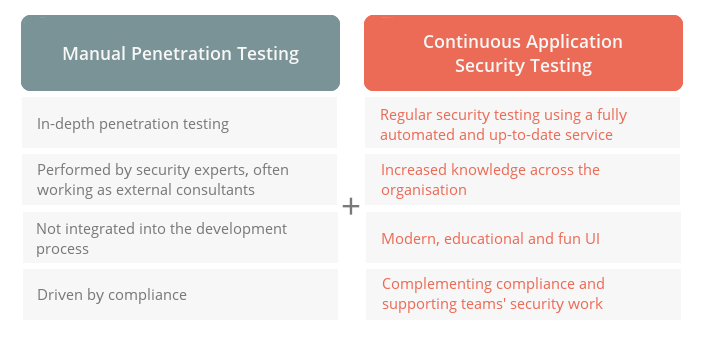
\includegraphics[scale = 0.6]{images/Automation_pentesting.png}
    \caption{\href{https://blog.detectify.com/wp-content/uploads/2017/08/Automation_pentesting.png}{Source. }Main differences between automated and manual audit}
\end{figure}

Also, it was required to know which attacks are the most common and the most lethal for companies and websites in general. The scope of the project was to cover the main vulnerabilities, even though it is aimed to be extended in the future to cover as many vulnerabilities as possible. \\It was mandatory to limit the number of tools and breaches covered in order to keep a portable code and also to limit the time of execution (since automated tools are "blind", it is sometime really long to execute the whole script). The main things that was identified among regular web vulnerabilities where XSS (Cross site scripting, injecting of Javascript code in certain input fields) SQL injections (requesting a database in a way that was not intended by the developer) and info leaks as backup files or else\cite{vuln}. These are the breaches that the tool will try to detect and exploit if possible. Other vulnerabilities that can be think of are irregular file uploads, local file inclusion or remote file inclusion, Cross Site Request Forgery but also command injection for example (this list is not exhaustive at all).

\begin{figure}[h]
    \centering
    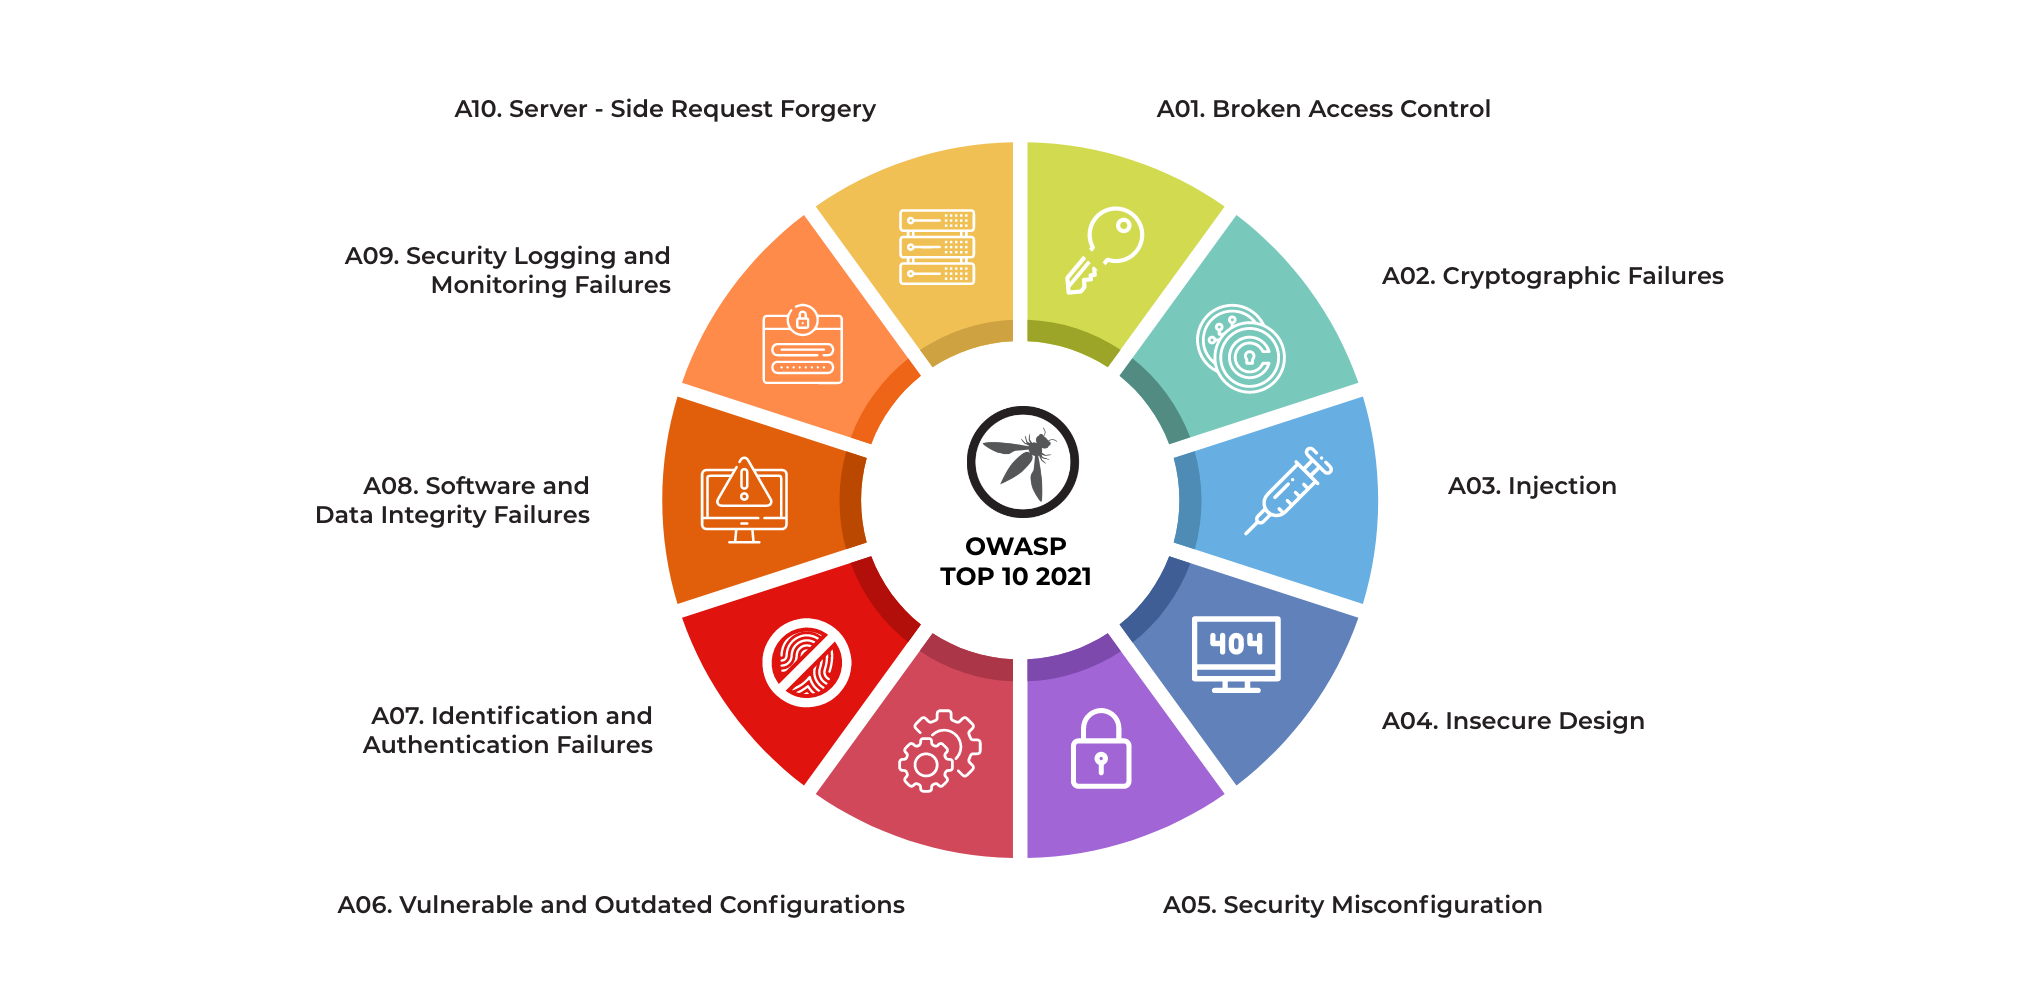
\includegraphics[scale = 0.23]{images/Infographic - OWASP Top 10 2021.png}
    \caption{\href{https://prismic-io.s3.amazonaws.com/horangiweb/22887c0e-2492-421f-8bbf-bdcb7fac4b5f_Infographic+-+OWASP+Top+10+2021.png}{Source. }OWASP Top 10 of most common breaches}
\end{figure}

The type of penetration testing is also important to choose\cite{type}. Indeed, a white box testing (which is an audit with the code available) is really different from a black box testing (when an outsider tries to hack). The most simple automated type of test to conduct is black box testing, because otherwise one have to go into code analysis and it can become out of hand and specific really fast. Knowing this, black box testing was chosen as it is the main one performed by usual tools and that it is a common scenario during web hacking (but maybe not the main one since insiders attacks are really more frequent than one can think). Also, it is important to underline that even though it is a big part of hacking and it is important to test it, social engineering is not covered by this paper. This could however be automated by spam bots and false emails for example, but this field is more about human skills than technical skills so this paper will not deal with it.
\\

\subsection{Finding a vulnerable app}

The first requirement to be able to test things on a virtual lab is to find a vulnerable web application to attack. There are many web applications already made that are available. This part has been a struggle because the writing of the Ansible scripts required no interaction and no input from the user at all. \\
The first web application that was chosen was \href{https://www.giac.org/paper/gwapt/3387/introduction-owasp-mutillidae-ii-web-pen-test-training-environment/126917}{mutillidae} because it is covering many vulnerabilities and it is suppose to be easy to deal with. However, the setup of the database was complicated and too many errors showed up, which were complicated to fix in a reasonable time. \\
Accordingly, another app had to be chosen. Google Gruyere seemed to be an interesting choice. The setup is easy and was realized using Ansible (the code is still available in the along CD). The problem with Google Gruyere was that it is really made for manual penetration testing and it was really complicated to get a decent automated testing on this app. Also, the documentation about this web application was not that exhaustive, so the project could not use this application either. \\ 
This paper\cite{webapps} is dealing with the subject of educational vulnerable websites deeply, and \href{https://www.giac.org/paper/gwapt/3387/introduction-owasp-mutillidae-ii-web-pen-test-training-environment/126917}{DVWA} (Damn Vulnerable Web Application) appeared to be the most easy and suitable option after reading this. Indeed, the setup is doable and building an Ansible script was possible. The app needed few modifications to be suitable for automatic penetration testing. Indeed, the login page was removed in order to get rid of the session id parameter which required human interaction. \\
This website has three levels of security, low, medium and high. The low level was chosen to be able to test as many things as possible. The available breaches are multiple and the XSS and SQL injection are part of them so the tool will be tested.

\begin{figure}[h]
    \centering
    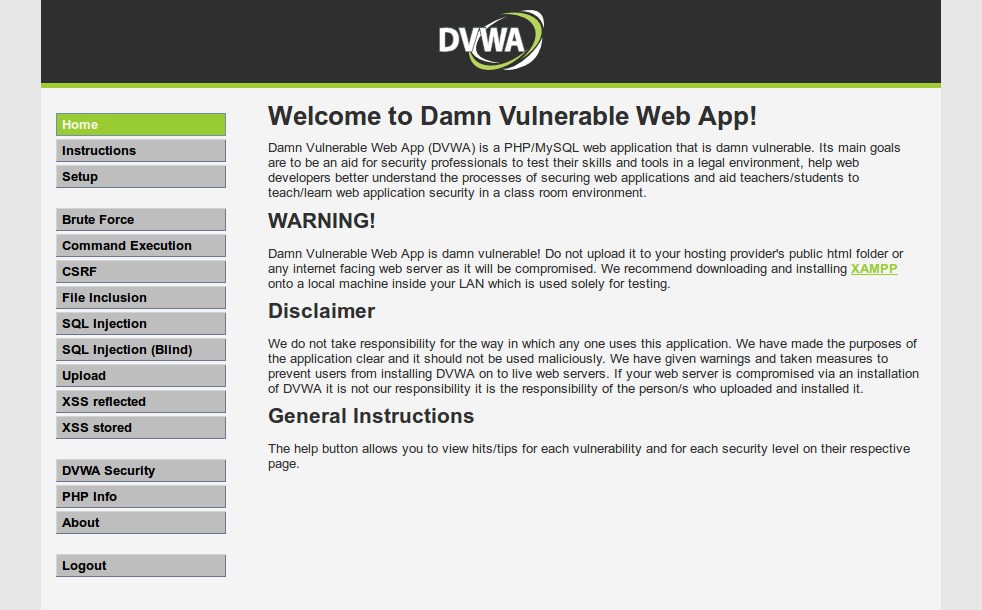
\includegraphics[scale = 0.45]{images/DVWA.png}
    \caption{\href{https://1.bp.blogspot.com/-UfcDBmOv8yk/WnI1MIxfopI/AAAAAAAAKHU/CDyhAkrVnbQWXWPh0BDr1bxmX8tA_fX0ACLcBGAs/s1600/DVWA.png}{Source. }The welcome page of DVWA}
\end{figure}

\subsection{The detection part}

The project also had to include a detection/report part in order to block or prevent such attacks. This paper\cite{detection}, even if old, give an overview of what means are possible to take in order to detect attempted hacking. However, this is mainly theoretical and now that new tools are available, there are multiple things to do. The first thing that comes to mind could be using \href{https://www.fail2ban.org/wiki/index.php/Main_Page}{fail2ban} or such software in order to block malicious IPs and that is the most logical thing to do. However, in the idea of trying to develop a script that would be deployed along the script that runs the server, a minimal python script was developed. The purpose of this script would be both to block weird or malicious looking requests, but also prevent a single machine to run a lot of queries in a short period of time to block bots and automated tools. In order to do this, there is a ban list that will not allow certain IPs to  

\section{Creation of the lab}

\subsection{Creation of the victim machine}

First of all, a victim machine is required in order to attack it and open it. There was many machine that could have been used to do this, has seen previously. It could have been possible too to develop a vulnerable machine but it would have take to long to do an exhaustive machine. Therefore, the victim machine had to be a server for an already existing vulnerable application.

\subsubsection{Mutillidae}
 
 The first option taken was Mutillidae, a web application developed by OWASP in order to help people train about hacking. However this web application did not work properly with the Ansible scripts and it was really complicated to debug things and to interact with the website (at this point the SSH tunnel was not working either so the comprehension of what was happening was minimal). Also, this web application relied on XAMPP, which had a lot of problem of compatibility when trying to install with Ansible and the whole installation was painful as time was running by. Mutillidae was abandoned, seeking for something more easy and flexible.

 \subsubsection{Google Gruyere}

Google Gruyere is a web application also developed for educational purposes, trying to show usual vulnerabilities to help people understand them and also allow to fix some of those. The installation is quite simple as it is relying on Python HTTP server module. The Ansible script is still available and is functional to install Google Gruyere. However, once installed and ready, during the testing of the attack scripts, it was clear that this option was not suitable at all because it has been made for manual penetration testing, most vulnerabilities are common ones but not properly exploitable by a machine without being specific. At this point, the web application was not interesting anymore for the purpose of this project so it was abandoned.

\subsubsection{DVWA}

Finally, DVWA (Damn Vulnerable Web Application) was the easiest and most complete option. Indeed, this web application developed for educational purposes too work with PHP and MySQL. After a few tutorial about the installation and some correction, the application is ready to be used. The login page had to be dropped, which was done by a simple modification in a configuration file, and then it was possible to query the application successfully with cURL first, and then with a python script. The whole process was mostly about taking care of Ansible fragile syntax and to correct some deprecated version of software. Dealing with regular expressions to modify files was also difficult sometimes.
\\
Also, since the machine has been created to get hacked, it is not a problem that it is on the university network because nothing sensitive is in there. However, one must be careful when installing such application on his computer because it can be an entrance point for an attacker, so one should never post DVWA online.

\subsection{Creation of the attacker machine}

\subsubsection{The tools}

When the defense machine was ready, it was time to create the attacker machine. In order to do so, the first thing was to research the main tools used to do automated penetration testing. Since the targeted vulnerabilities where directory listing, SQL injection and XSS injection, it was easy to find such tools. Indeed, sqlmap is the reference\cite{sqli} in terms of automated tools for SQL injection, for the directory listing, dirb\cite{dirb} seemed to be the easiest option (dirbuster was tried before but it is the graphic version of the tool and cannot be used through the automation process because it requires input) even though the wordlist method is brutal and does not cover every folder or file. For XSS injections, a nice tool has been developed in Python called \href{https://github.com/pwn0sec/PwnXSS}{PwnXSS} that do everything that is required in the project. Also we needed to have a list of the URL to attack because some tools do not crawl websites properly. In order to build this, BeautifulSoup (a module that does html parsing) was used to gather every "href" tags and put them in the list (except for outside links). Nmap was required to make the script a bit more generic and to make sure we try every port that had http over it. It was used in the beginning of the script has the "discovery" part of the kill chain along with finding URLs to attack.

\begin{figure}[h]
    \centering
    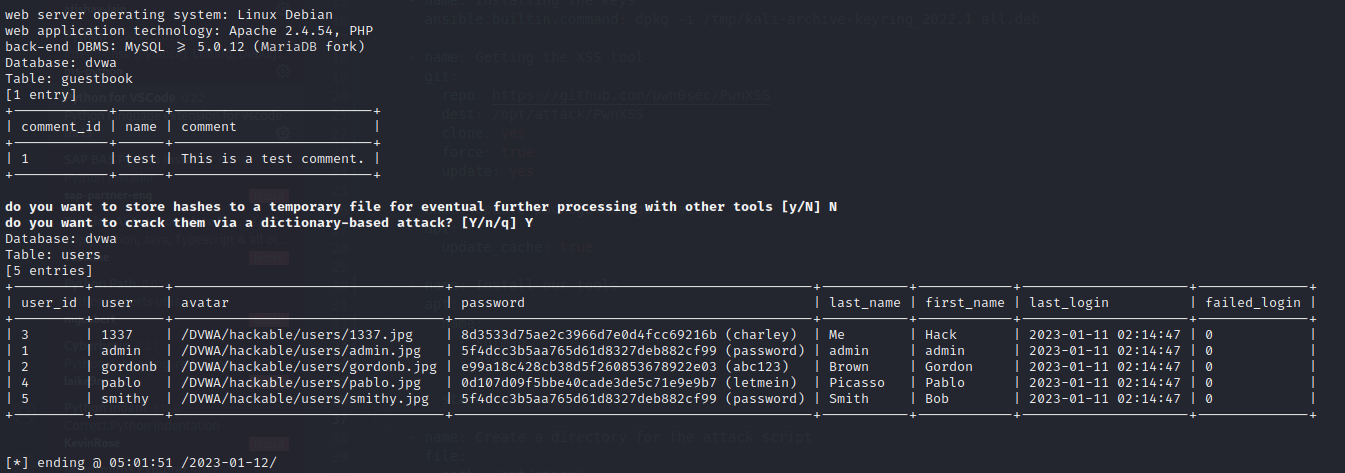
\includegraphics[scale = 0.3]{images/sqlmap.png}
    \caption{Some sqlmap output}
\end{figure}

\subsubsection{The setup}

In order to set this machine up, it was required to have access to the Kali Linux packages because dirb along with sqlmap and nmap are Kali packages. It was then required to add the Kali repository to our sources and to make the public key check in order for apt to be able to download these. One this was done, the packages needed to be downloaded along with PwnXSS which is accessible on Github. Then the script needed to be copied from our host machine to the remote host, with installing all the requirements and setup the whole virtual environment to make sure not to interfere with anything else on the machine.

\begin{figure}[h]
    \centering
    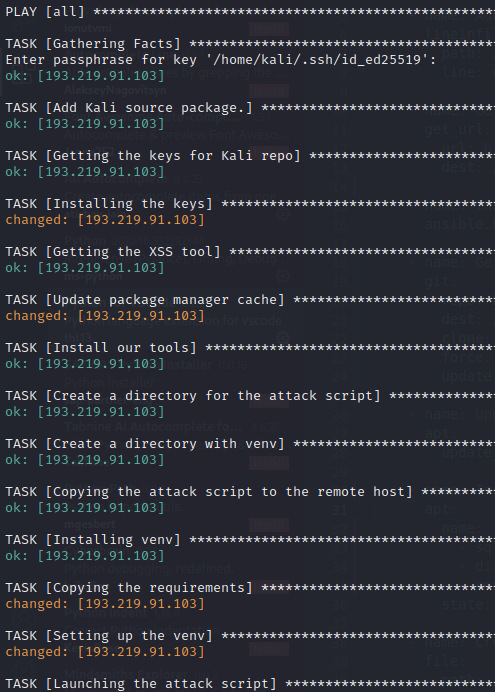
\includegraphics[scale = 0.6]{images/attack_install.png}
    \caption{The Ansible playbook running}
\end{figure}

Unfortunately, Ansible does not have a feature to see the output during the execution of the code, therefore we have to wait until the whole process is done until seeing some output. However since the script is fast so far it is not that much of a problem.

\subsection{Creation of the detection script}

In order to create the detection script, it was required to build a ban list with the IP of the attacker that were spamming. However, building a script like this was far more complicated than expected and the project needed to be ended because most of the time has been consumed doing the setup of the vulnerable machine, this topic was not extended. However, things will be explained in the next part of this paper.

\section{Experiences and test}

Since the lab was ready, it was time to do some testing. The result expected where a list of directory that were found by dirb, information about the database given by sqlmap and also pages that were sensitive to XSS. Along with that, the expected result was also a list of URL that could be queried in order to find vulnerabilities.

\subsection{Dirbuster}

For the dirb tool, the result was a list of file and directories that could be accessed freely by the user. However, the output of dirb is not really suitable because it is really verbose, so it was required to use the "-S" option in order to have less output. Even with this option on, there was still too many information so the output was scrapped in order just to keep the filenames. At first, the requested host was "http://10.0.0.64" only, without specifying the /DVWA folder. In this configuration, the output is not really great. However, if we do specify the folder we can gather a few files and directories.

\begin{figure}[h]
    \centering
    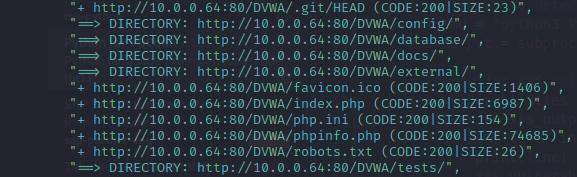
\includegraphics[scale = 1]{images/dirb.png}
    \caption{The scraped output of dirb}
\end{figure}

We can still notice that not every folder has been found there, because the way dirb functions is really simple. Dirb has a wordlist with candidate folders or file names, and he just requests the website with these. If he gets a 404 error, the file or folder doesn't exist, if he have something else he add it to the list. The problem with these methods is that it is not discreet at all, but also it cannot find every directory because if the name is not in the wordlist it will not be find. That is why a few lines of Python have been added to gather the href attributes around.

\begin{figure}[h]
    \centering
    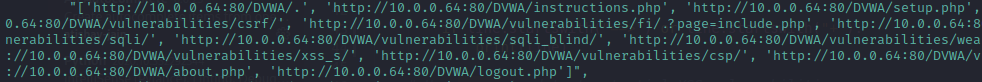
\includegraphics[scale = 0.6]{images/href.png}
    \caption{Part of the list of collected hrefs}
\end{figure}

\subsection{SQL}

The SQL injections are the one that did not work out really well. Indeed, sqlmap requires that the user give the injectable parameter in order to find the breach and to dump the table. This specific URL was found and added in the script, but this was not intended like this because the software is now less automated than it should be. Indeed, if the user has to manually enter the good URL, it is not really automated. Even with the crawl parameter set properly, sqlmap cannot fin the injection itself and is also really slow when checking every URL for injection. However, when the id is provided sqlmap is really fast and give every needed information about tables. To keep the script fast only the --dump option is used and not the -a (that would really give each tables in the database) because it is already some interesting dump to see and as a proof of concept. Also notice that the --batch is used; this option allows the tool to work on its own without asking for inputs. Only default values are used. Also, sqlmap is able to crack vulnerable hashes on its own and does it pretty fast. For an unknown reason, sqlmap is overly verbose in the Ansible execution while it is completely quiet when executing the same command outside the playbook. Cracking the passwords looks to be a problem. This behavior was not expected and may be related to the way Ansible deal with terminal command launching

\begin{figure}[h]
    \centering
    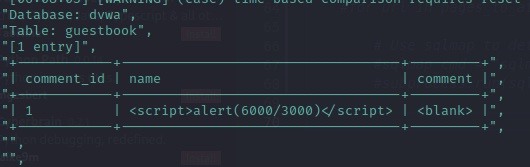
\includegraphics[scale = 1]{images/sqlxss.png}
    \caption{Sqlmap retrieve a table damaged by XSS injection}
\end{figure}

\subsection{XSS}

XSS injections were scary at first because the same problem than with the SQL injection could occur. However, the PwnXSS tool is really well made and crawl the website without any problems. Therefore, it was easy to find a way to exploit it to output the vulnerable URLs that could be attacked with XSS. With the crawl parameter set properly, the whole website is traveled and every XSS is found, except the DOM one for an unknown reason (maybe PwnXSS does not cover them). Anyway, once the output is scraped there is a really nice list of vulnerable path with the way of attacking them.

\begin{figure}[h]
    \centering
    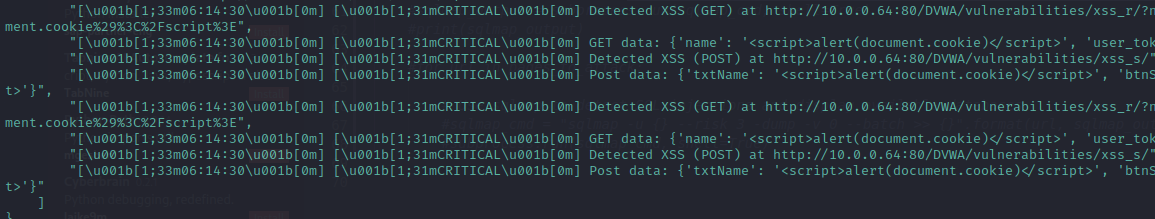
\includegraphics[scale = 0.5]{images/xss.png}
    \caption{The XSS injections discovered in DVWA}
\end{figure}

\subsection{The detection script}

The detection script was based on the idea of listening the incoming traffic on the same port as the web server in order to intercept requests. However we cannot do that with Python without making some port redirection or by using another tool like netcat or tcpdump. Even with those tools, it was complicated to code what was required so this project does not cover this part properly. However, the idea was to check the request sent by the outside and to trigger some ban when the URL looked suspicious, with SQL related character or script tag for example. The idea was also to ban IP that were querying the server too fast but I had no idea how to do that and was running short on time.


\subsection{The overall result}

The overall result is a victim machine (more than a defensive one since detection is off) configured properly with an attacking script that is able to hit and to gather some information by using regular tools. Discretion is not on, but the script is able to collect directories and files, database dumps and XSS vulnerabilities in a decent timing. 

\begin{figure}[h]
    \centering
    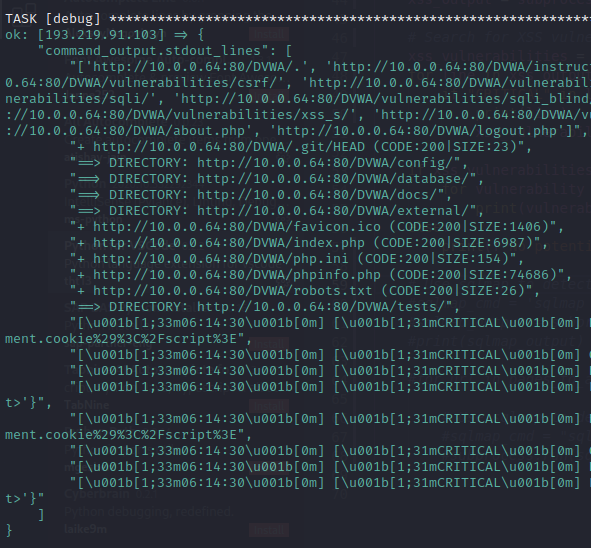
\includegraphics[scale = 1]{images/general.png}
    \caption{The result of the attacking script}
\end{figure}

\section{Ideas for improvement}

\subsection{Detection}

To improve this project the detection part could be really interesting. The usage of fail2ban could be a nice way to do it without custom scripts, and it may be really fast and easy because the software is still updated to this day and has a good reputation.

\subsection{Other tools}

There are many vulnerabilities that are not covered by the attacking script such as Local File Inclusion, OS code injection, CSRF, File upload and others. There was some attempt to cover Local File Inclusion and OS code injection with tools already available. For LFI (Local File Inclusion), there is a file called LFISuite\cite{LFI} but it requires too many interactions with the user to be used in an automated process as it is right now. An interesting topic would be to modify the code in order to have a batch mode like in sqlmap for example. For OS code injection, a software called commix\cite{OSinjection} is popular. It is supposed to work with DVWA, but it seems that some updates made it unreliable on DVWA because it cannot find the OS injection even when the parameters are specified. If it worked it would have been easy to add it in the attacking script.

\begin{figure}[h]
    \centering
    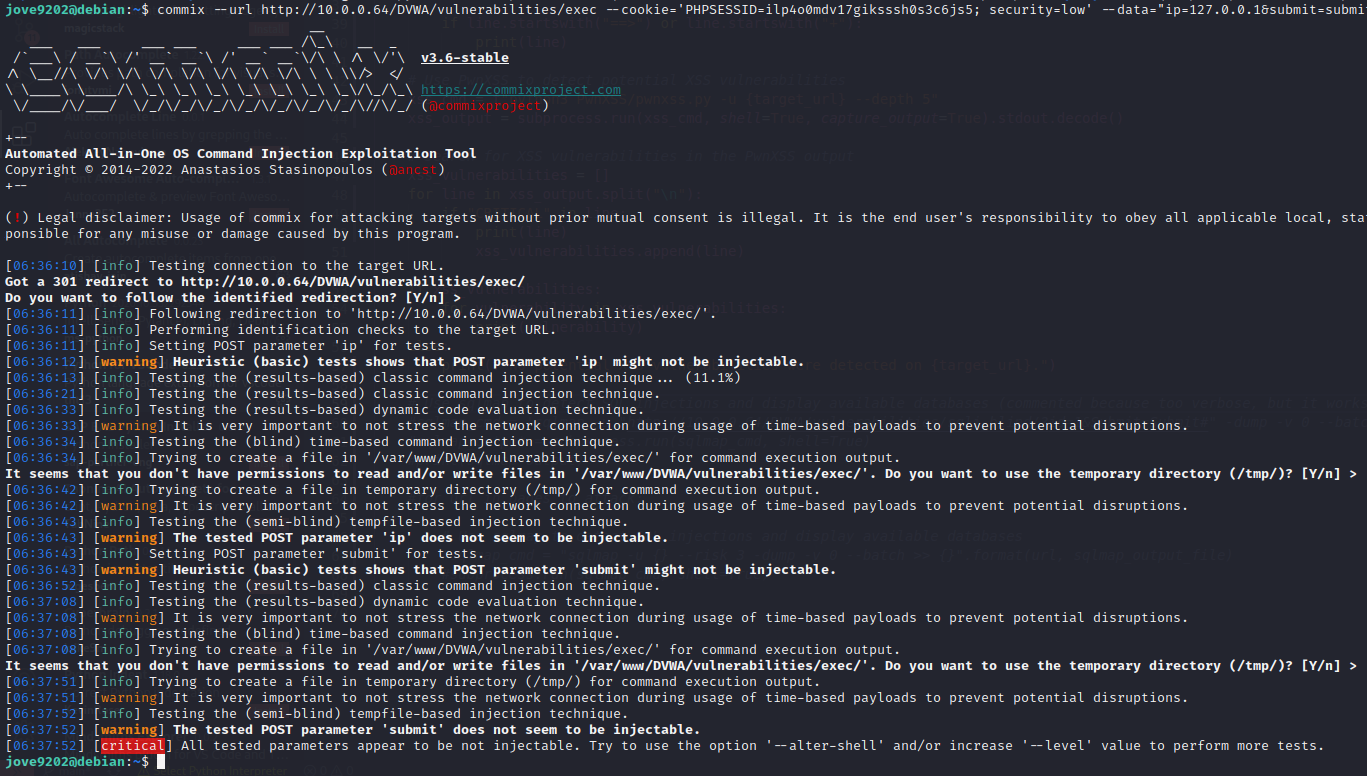
\includegraphics[scale = 0.4]{images/commix.png}
    \caption{The result of the usage of commix in DVWA}
\end{figure}

Also, to correct the problem in the SQL a parameter miner could be useful in order to be able to gather the potentially injectable parameter directly in the script. However, both tools that were tried during this project were not able to find a single parameter in DVWA even though there are plenty. Both Arjan and ParamSpider have been tried but no interesting result came out.

\begin{figure}[h]
    \centering
    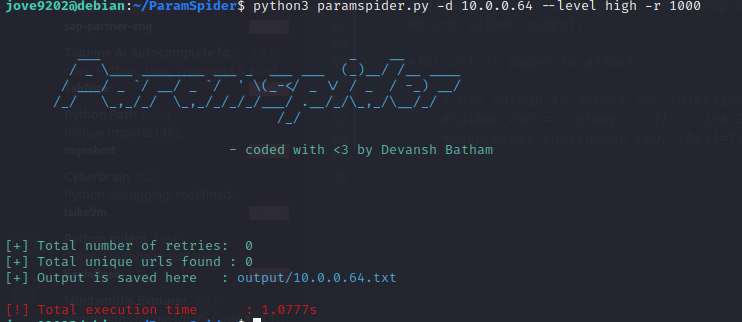
\includegraphics[scale = 0.7]{images/param.png}
    \caption{The result of the usage of ParamSpider in DVWA}
\end{figure}

Finally, some poweful tools suck as nikto for example could be used to really test the entire website. However, since it seems that these tools are actually the aim of this project, it was not fair to use it there, but for future purpose it could be an interesting idea.

\subsection{General coding}

The main problems remaining with the code (that actually could be fixed easily) would be to add a parameter to the attack script to be able to change the host quickly. A makefile could also be done in order to launch both setups in the same time, that would be faster than the current organization. The Ansible script could take a parameter for certain things as the source folder from which we copy things, but that could be a bit heavy.



 %Conclusions section
\sectionWithoutNumber{\keyWordConclusions}{conclu}
To conclude, this project is not well finished yet and require some improvements to be really exhaustive. However, it offers a base to start from with an easy and fast way to set up a cybersecurity lab in order to do some training for academic purposes. The automation of penetration testing is already a big concern in the cyber industry and most professionals use tools like Nessus to find the most common CVE with a web interface that allows them to know straight away the level of vulnerabilities that they will find on the attack surface. However, the approach of this project is mostly educative, therefore the CLI tools and the description of what is happening is interesting to understand what is happening and why, even though the best way to do that is by going manual. The detection part looks a bit harder because it implies some network knowledge and it seems to be difficult to code by itself, however it definitely could be achieved. There are a lot of open source tools on internet and checking the code and modifying it to meet the need of this project could definitely be interesting even if time consuming. \\

For the personnal part, I would say I really enjoyed this project because it was interesting mostly to play around with ansible but also to discover new tools, however I think I do not have enough knowledge about the tool I used to make them all work properly.

 %file literatureSources.bib
\referenceSources{literatureSources}

\newpage
\begin{appendices}

\newpage
\section{Github link}
\label{app:a}
The source code is available at \href{https://github.com/JoannVetter/Attack-defense-automation}{this GitHub link}.
\end{appendices}

\end{document}
